\documentclass[12pt]{article}

\usepackage{listings}

\usepackage{comment}
\usepackage{subcaption}

\usepackage[margin = 1in, left = 1.5in, includefoot] {geometry}

%Adding Image
\usepackage{graphicx}
\graphicspath{{images/}}

%HyperLinks for Table of Contents
\usepackage[hidelinks]{hyperref}
\hypersetup{colorlinks = true, citecolor = black, linkcolor = blue, urlcolor = black}

%Title
%\title{\textbf{Embedded Systems \& IoT\emph{ \\Course Report}}\\}

%\usepackage{helvet}%Bookman Font

%Starting of the Document
\begin{document}

\begin{titlepage}

	\begin{center}
	
	\line(1,0){350} \\
	[0.25in]
	\huge{\bfseries Embedded Systems \& IoT \\Course Report} \\ [1mm]
	\line(1,0){200}\\
\begin{normalsize}
	\textbf{{\large \\Sai Krishna Dasari\\}}
	{\large Trainee, Group-3 ES}{\large , SURE Trust\\}
	 November 2022 - February 2023
\end{normalsize}

	%\maketitle
	%[0.1cm]
	
	%by\\
	
	%\textsc{\Large Internship Report on Technology Commercialization in India \& Germany} \\
	
\begin{figure}[h]
\centering

\includegraphics[scale=0.9]{suretrust_logo.png}
\end{figure}

\textbf{\LARGE {THE SURE TRUST}} \\
\href{https://suretrustforruralyouth.com/}{Skill Upgradation for Rural youth Empowerment  TRUST}\\
\begin{normalsize}
\textbf{\textbf{\\Trainer}}\\
\textbf{Mr. Yogesh Kumar} \\
B.Tech (ECE)\\
Technical Presales Consultant \\ ThirdEye AI Pvt Ltd\\
\end{normalsize}

	\end{center}
	

\end{titlepage}

%\maketitle %Title will go over here




\pagebreak

\begin{figure}[h]
\centering

\includegraphics[scale=0.6]{suretrust_logo.png}
\end{figure}

\begin{center}
{\LARGE \textbf{ Declaration\\}}
\end{center}
%\vspace{0.5in}
{\large  \hspace{0.6in}     This is to certify that \textbf{Sai Krishna Dasari} has successfully    completed the\textbf{ four months} training given in “\textbf{Embedded Systems and Internet of Things conducted by The SURE TRUST}” during the period from \textbf{November 2022} to\textbf{ February 2023}}.\\

{\begin{center}
\begin{figure}[h]
\centering

\includegraphics[scale=0.6]{yogeshsir_sign.png}
\end{figure}
\textbf{Mr.Yogesh Kumar}\\
Trainer,\textbf{SURE Trust}
\end{center}}

\begin{figure}
  \begin{subfigure}[b]{0.4\linewidth}
    
\includegraphics[width=\linewidth]{radhamam_sign.png}
    \caption*{\textbf{Prof. Ch. Radha Kumari}\\
 Executive Director \& Founder\\
 \textbf{SURE Trust}}
    \label{fig:image1}
  \end{subfigure}
  \hspace{0.2\linewidth}
  \begin{subfigure}[b]{0.4\linewidth}
    
\includegraphics[width=\linewidth]{vandana_sign.png}
    \caption*{\textbf{Mrs. Vandana Nagesh}\\
Trustee \& Advisor\\
 \textbf{SURE Trust}}
    \label{fig:image2}
  \end{subfigure}
  \label{fig:two_images}
\end{figure}

\begin{comment}
{\begin{flushleft}
\begin{figure}[h]

\includegraphics[scale=0.8]{radhamam_sign.png}
\end{figure}
\textbf{Prof. Ch. Radha Kumari}\\
 Executive Director \& Founder\\
 \textbf{SURE Trust}
\end{flushleft}}
 \hspace{0.6in}
{\begin{flushright}
\begin{figure}[h]
\begin{flushright}

\includegraphics[scale=0.6]{radhamam_sign.png}
\end{flushright}
\end{figure}
\textbf{Prof. Ch. Radha Kumari}\\
 Executive Director \& Founder\\
 \textbf{SURE Trust}
\end{flushright}}
\end{comment}

\pagebreak
\tableofcontents %for making table of contents
\clearpage

\begin{center}
\section*{\textbf{THE SURE TRUST}}
\addcontentsline{toc}{section}{1. THE SURE TRUST}
\end{center}

\subsection*{Introduction to The SURE TRUST}
\addcontentsline{toc}{subsection}{Introduction to The SURE TRUST}
The SURE TRUST is born to enhance the employability of educated unemployed rural youth. It is
observed that there is a wide gap between the skills acquired by students from the academic
institutions and the skills required by the industry to employ them. Employability enhancement is
done through giving one on one training in emerging technologies, completely through online
mode.

 The mission of the SURE TRUST is to bridge the gap between the skills acquired and the skills
required by training them in the most emerging technologies such as Artificial Intelligence (AI),
Python Program, Machine Learning (ML), Deep Learning (DL), Data Science \& Data Analytics,
Blockchain Technology, Robotic Process Automation (RPA), Project Management, Excel for Business
Application, Statistical tools \& Applications, Spoken English and Business Communication etc., that
will enhance their employability. 

After completion of four months training in the course, the trainees will get live projects from industries as internship activity to get experience in applying to real time situation what they have learned during the course. These projects will give them hands on experience which is much sought after by the prospective industry employing them. Currently students from all over India are enrolling for various courses offered by the SURE TRUST. The SURE TRUST offers every course free of cost with no financial burden of any kind to students.

 This initiative is purely a service-oriented one aiming to guide the rural youth who are educated but unemployed due to lack of up-gradation in their skill sets. The birth of SURE TRUST is a God given boon to rural youth who could reach great heights either in employment or in entrepreneurship once they receive the training offered followed by the company internship. Many companies are coming forward to join their hands with us by offering internship projects to hand hold and lead the rural youth in their career settlement.
 
 \subsection*{Vision of the SURE TRUST}
 \addcontentsline{toc}{subsection}{Vision of the SURE TRUST}
 The vision of the SURE TRUST is to enhance the employ-ability of educated unemployed youth,
particularly living in rural areas, through skill up-gradation, with no cost to the students.

 \subsection*{Mission of the SURE TRUST}
 \addcontentsline{toc}{subsection}{Mission of the SURE TRUST}
The mission is to bridge the gap between the skills acquired in the academic institutions and the
skills required in industries as a pre-condition for employment.

 \subsection*{Functioning of the SURE TRUST}
 \addcontentsline{toc}{subsection}{Functioning of the SURE TRUST}
There are three dedicated, committed, and hard-working women on the board of management
of the SURE TRUST who will look into the various administrative and other matters relating to
the enrollment of students, organizing trainers, entering into agreements with companies for
getting live projects to students as internship programs, and so on. All the three women on the
board are all the alumni from Sri Sathya Sai Institute of Higher Learning, Anantapur Campus,
deemed to be a University. The women board is supported by five eminent advisories who are
from different walks of life and have made outstanding mark in career in their respective fields.
For more details about SURE TRUST please visit the website \href{https://suretrustforruralyouth.com/}{ www.suretrustforruralyouth.com}.

\section*{Course Content}
\addcontentsline{toc}{section}{2. Course Content}
The SURE TRUST conducts four months of training for every course on a uniform basis. A session
spanning across one to one \& half hour is taken by the trainers for every major course. Sessions
are conducted to complete the predesigned course structure within a fixed time period. Course
content is designed to suit the current requirement of the Industry and validated by industry
experts. The course content of all these courses is so dynamic that any changed condition
noticed in the industry will automatically get reflected in the content of the respective course.
As the course content is dynamic, the Following is the course content of the current course in
\textbf{Embedded Systems and Internet of Things}:

\pagebreak

\begin{center}
\section*{Embedded Systems and IoT} 
\addcontentsline{toc}{section}{3. Embedded Systems and IoT}
\end{center}

 \subsection*{Objective}
 \addcontentsline{toc}{subsection}{Objective}
This Course can make the learners build Embedded systems, IoT applications, and
projects which are being part of smart cities.

 \subsection*{Course Content}
 \addcontentsline{toc}{subsection}{Course Content}
This Course can make the learners build Embedded systems, IoT applications, and
projects which are being part of smart cities.

\subsubsection*{Module 1: Introduction to Embedded System}
\addcontentsline{toc}{subsubsection}{Module 1: Introduction to Embedded System}
\begin{itemize}
  \item Understanding what is Embedded System?
  \item Components of Embedded System
  \item Difference between Microprocessor and Micro controller
   \item Who plays the important role in Embedded system and how?
\end{itemize}

\subsubsection*{Module 2: Basic Electronics}
\addcontentsline{toc}{subsubsection}{Module 2: Basic Electronics}
\begin{itemize}
  \item Basic Terms used in Electronics Understanding all of them
  \item Analog and Digital
  \item Embedded System Architecture
   \item Instruction Sets
\end{itemize}

\subsubsection*{Module 3: Micro controller}
\addcontentsline{toc}{subsubsection}{Module 3: Micro controller}
\begin{itemize}
  \item Short introduction to 8051(The first Micro controller)
  \item Different Types of Micro controller
  \item Internal Main Components of Micro controller
   \item Development Boards
\end{itemize}

\subsubsection*{Module 4: Understanding the Arduino (ATMEGA328)}
\addcontentsline{toc}{subsubsection}{Module 4: Understanding the Arduino (ATMEGA328)}
\begin{itemize}
  \item Basics of Digital Circuits
  \item Understanding Arduino pin out
  \item Understanding Arduino IDE
   \item Learning Arduino Embedded C Commands
\end{itemize}

\subsubsection*{Module 5: Working on Projects}
\addcontentsline{toc}{subsubsection}{Module 5: Working on Projects}
\begin{itemize}
  \item Automatic Speed Control of motor depending upon temperature.(Learning the role of PWM)
  \item Turning on and off the device by clapping
  \item Smart Surveillance System using GSM 
   \item Solar Tracking System
   \item Automatic Hand Sanitize Machine 
   \item Understanding Conveyor assembly used in Industries and building small project on it
   \item Real Time Based system using RTC module for schedule operation
   \item Solar power Monitoring using LCD
   \item Close loop Control system based project 
   \item Over Voltage and Over Current protection system
   \item Radar System mini project to understand how it is in important in defense sector
   \item More projects related to the industries as per students interest
\end{itemize}

\subsubsection*{Module 6 : How to design our own Embedded System}
\addcontentsline{toc}{subsubsection}{Module 6 : How to design our own Embedded System}
\begin{itemize}
  \item Parameters to look while designing and choosing components
  \item Introduction to DIP-TRACE Circuit designing Software
  \item Few Designing examples
   \item Discussion on product development
\end{itemize}

\textbf{Note:}All the projects and topics will be explained by providing real life example for better understanding of concepts.

 \subsection*{Conduct of the Course}
 \addcontentsline{toc}{subsection}{Conduct of the Course}
 
Modalities for the conduct of all the courses are fixed by the SURE TRUST which are uniformly followed across the courses.\\

 \begin{flushleft}
 Mode of Training --- Online\\
 Period of Training --- Four months\\
 Sessions per week --- 3 to 6\\
 Length of the session --- 1 to 2 hours\\
 Tests to be taken --- 2 per month\\
 Assignments --- 2 per month\\
 Last 15 days --- Final practice and preparing the course report\\
 \end{flushleft}
 \subsection*{Student Byelaws}
  \addcontentsline{toc}{subsection}{Student Byelaws}
 
Students enrolling for the courses under SURE TRUST are strictly required to follow the following Byelaws set for them.
 
\begin{flushleft}
\textbf{ Note:}Byelaws for students to become eligible for certificate at the end of the course
\end{flushleft}
 \begin{itemize}
  \item \textbf{Minimum Attendance:}
 
  Every student must put in a minimum of 85\% attendance in attending the classes for getting the
  eligibility to receive the certificates.

  \item \textbf{Two written tests are to be taken each month:}
  
  Since the objective of the certification program is to turn out well-qualified students from the respective courses, minimum two written tests are to be taken in each month for each course to ensure that the students are pulled along the expected line of standard.
  
  \item \textbf{Assignment submissions:} 
  
Ten exercises constituting one assignment for every two to three new functions/topics taught, resulting in minimum seven such assignments are to be submitted during the four months period.  
  
   \item  \textbf{Preparing the final course report in the prescribed format:}
   
   During the last fifteen days in the fourth month, students many be asked to consolidate and compile all the assignments submitted in a word document along with the other chapters which will constitute a course report for each student. This report will be the unique contribution a student carries from the trust to showcase the rigorous training he/she received during the four months period. Besides the report will stand as a testimony to the detailed learning a student has acquired in the chosen area. This will facilitate the industry in handpicking the required student for the job.

   \item \textbf{External Viva-voce:} 
   
   Every student has to successfully clear the external viva-voce arranged in their respective course.
   
   \item \textbf{KYC norms:}
   
   Each student wishing to enrol for the course must submit a written letter saying that he/she will not drop from the course until its completion, which will also be signed by father / mother besides the student himself / herself.
   
   \item \textbf{Attend the full class:}
   
   All the students are expected to attend each class for full duration. Some students are observed moving out of classes after logging in which does not go well with the learning objective of students.

   \item \textbf{Ensure discipline in the group:}
   
   All the students are advised strictly to follow group etiquette and restrain from posting in the group any unethical messages or teasing messages or personal interactive messages. This group is purely created for academic purposes and hence only academic interactions should go on. 

\end{itemize}
\pagebreak
 \begin{center}
   \section*{EACH ONE PLANT ONE}
    \addcontentsline{toc}{section}{4. EACH ONE PLANT ONE - {\normalsize An Initiative By SURE Trust}}
  ( An Initiative By SURE Trust)
  \end{center} 
  The "\textbf{Each One Plant One}" initiative is one of the many programs conducted by the SURE Trust, aimed at promoting \textbf{sustainable development} and \textbf{environmental conservation} in rural India.
  
   The initiative is based on the simple principle that if \textbf{every person plants one tree}, the collective impact can be significant in terms of combating deforestation, air pollution, and climate change.

Through the "\textbf{Each One Plant One}" initiative, the \textbf{SURE Trust} seeks to encourage the planting of trees among individuals, organizations, and communities in rural areas.
  
The program emphasizes the importance of trees in mitigating the effects of \emph{climate change}, \emph{improving air} and \emph{water quality}, and providing \emph{habitat for wildlife}. In addition to these benefits, tree planting also contributes to \textbf{food security}, as some trees provide fruits, nuts, and other products that can be consumed or sold.

The "\textbf{Each One Plant One}"[Fig:\ref{each_one_plant_one}] initiative is an excellent example of a community-led environmental initiative that promotes sustainable development and empowers rural communities to take ownership of their natural resources. By promoting tree planting and environmental conservation, the SURE Trust is helping to create a more resilient and sustainable future for rural India.\\

\begin{figure}[h]
\centering

\includegraphics[scale=0.7]{eachoneplantone.png}
\caption{\textbf{Each One Plant One}}
\label{each_one_plant_one}
\end{figure}

\begin{center}
\section*{{\large Embedded Systems and IoT \\ PROJECTS}}
 \addcontentsline{toc}{section}{{\large PROJECTS}}
 \section*{PROJECT - 1}
\section*{\textbf{Password Protection Using Push Buttons}}
 \addcontentsline{toc}{section}{1. Password Protection Using Push Buttons}
\end{center}

\subsection*{\textbf{Description :}}
 \addcontentsline{toc}{subsection}{Description}
 This Project is to design a system using Arduino UNO containing push button as keys from 0-9 Numbers which are inputs for Arduino when user enters Correct password using push buttons then Green LED need to ON and Welcome message will be displayed in LCD display. If user enters wrong password then he can attempt another time. If the number of attempts exceeds more than 3 times then buzzer need to blow and warning message will be displayed in LCD display and Red LED need to ON.\\ 
 
 
 \subsection*{\textbf{Block Diagram :\\}}
 \addcontentsline{toc}{subsection}{Block Diagram\\}
 
 \begin{figure}[h]
\centering
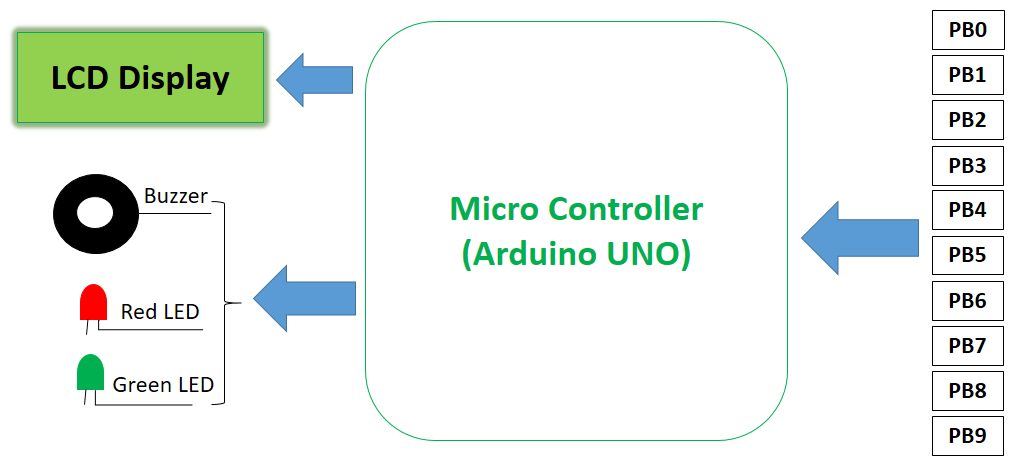
\includegraphics[scale=0.5]{block1.png}
\caption{\textbf{Block Diagram}}
\label{block_diagram1}
\end{figure}

\pagebreak

 \subsection*{\textbf{Input and Output :}}
 \addcontentsline{toc}{subsection}{Input and Output}
 
 \begin{tabular}{|c|c|c|c|c|c|c|}
  \hline
 \textbf{S.No }& \textbf{Description} & \textbf{Name}&\textbf{Type }& \textbf{Data Direction}  &\textbf{ Spec}& \textbf{Remarks} \\
  \hline
  1 &  Push Button & PB0 & INP  & DI  &5VDC&Active High \\
  \hline
  2 & Push Button & PB1 &INP  & DI  &5VDC&Active High \\
  \hline
  3 &  Push Button & PB2 &INP &DI &5VDC&Active High \\
  \hline
  4 &  Push Button & PB3 &INP & DI  & 5VDC&Active High \\
  \hline
  5& Push Button & PB4 &INP &DI &5VDC&Active High\\
 \hline
  6 & Push Button & PB5 &INP &DI &5VDC&Active High \\
  \hline
  7 &  Push Button & PB6 &INP & DI  &5VDC&Active High\\
  \hline
   8 & Push Button & PB7 &INP  & DI &5VDC&Active High \\
  \hline
  9 & Push Button & PB8 &INP & DI &5VDC&Active High \\
  \hline
  10 &Push Button & PB9 &INP &DI &5VDC&Active High \\
  \hline
  11 & LCD Display & LCD &OUT & DI &5VDC&Active High \\
  \hline
  12 &  Red LED & LED1 &OUT & DO &5VDC&Active High \\
 \hline
  13 &  Green LED & LED2 &OUT & DO &5VDC&Active High \\
  \hline
  14 & Buzzer & BUZ &OUT& DO &5VDC&Active High \\
  \hline
\end{tabular}

 \subsection*{\textbf{Source Code :}}
 \addcontentsline{toc}{subsection}{Source Code}
 \begin{lstlisting}[language=C] 
#include <LiquidCrystal.h>
#include<string.h>

const int rs = A5, en = A4, d4 = A3, d5 = A2, d6 = A1, d7 = A0; 

LiquidCrystal lcd(rs, en, d4, d5, d6, d7);
unsigned int arduino_button_pins[]={0,1,2,3,4,5,6,7,8,9};
 
unsigned int button_past_values[]={0,0,0,0,0,0,0,0,0,0};

const int Green_LED=10;
const int Red_LED=11;
const int Buzzer=12;

int key_pressed() 
{

  for(uint8_t button=0;button<10;button++)
    {
      int present_state = digitalRead(arduino_button_pins[button]); 
      int previous_state= button_past_values[button];
      
      if(present_state)
      {
        if(present_state != previous_state) 
        {
          button_past_values[button] = present_state;
          char str[10];
          sprintf(str,"KEY:%d",button);
          lcd.setCursor(0,1);
          lcd.write(str);        
          return button; 
        }
      }
          
      else 
      {
        button_past_values[button] = 0; 
      } 
      
      delay(50);     
    }    
  
}

int press_button()
{
  if (digitalRead(0)||digitalRead(1)||digitalRead(2)||
         digitalRead(3)||digitalRead(4)||digitalRead(5)
        ||digitalRead(6)||digitalRead(7)||digitalRead(8)
        ||digitalRead(9)) 
  { 
    return 1; 
  }
  else
  { 
    return 0; 
  }
}

void setup()
{
  for(int i=0; i<10;i++)
  {
    pinMode(i,INPUT);
  }  
  pinMode(Green_LED,OUTPUT); 
  pinMode(Red_LED,OUTPUT);
  pinMode(Buzzer,OUTPUT); 
  lcd.begin(16, 2); 
  lcd.write("ENTER PIN"); 
}
  const int Preset_Pin=1111; 
  int pinByUser[] ={0,0,0,0} ;
  int keySequence = 0;
  int Final_Pin = 0 ;
  
void loop() 
{ 
   while(press_button()) 
    {
      if(keySequence<4)  
      {
         pinByUser[keySequence]=key_pressed();
         lcd.setCursor(6,1);
         char pin[4];
         sprintf(pin,"DIGIT%d-%d",keySequence+1,pinByUser[keySequence]); 
         lcd.write(pin);
      }

      else if(keySequence==4)
      {
          lcd.clear();
          lcd.write("ENTER PIN");                  
          lcd.setCursor(0,1);
          
          //generates inter pin from an Array(i.e. {1,2,3,4} ---> 1234)
          for(int a=0; a<4; a++)  
          {
            Final_Pin = (Final_Pin * 10) + pinByUser[a]; 
          } 
                  
         char pin[4];
         sprintf(pin,"PIN:%d",Final_Pin);
         lcd.write(pin);
         delay(1000);
        
        if(Final_Pin == Preset_Pin)
        {
          lcd.clear();
          lcd.setCursor(0,1);
          lcd.write("--CORRECT--"); 
          lcd.setCursor(0,0);
          lcd.write("ACCESS AUTHORIZED !!"); 
          digitalWrite(Green_LED,HIGH);
        }
             
        else 
        {
          lcd.clear();
          lcd.setCursor(4,0);
          lcd.write("Warning");          
          lcd.setCursor(3,1);
          lcd.write("-!FAILED!-"); 
          digitalWrite(Red_LED,HIGH);
        }            
      }
      
      else 
      {
        lcd.clear();
        lcd.setCursor(0,0);
        lcd.write("MAX LIMIT REACHED");
        digitalWrite(Buzzer,HIGH); 
      }
      
      delay(500);
      keySequence++;
    }         
}
 \end{lstlisting}
 
 \pagebreak
 
  \subsection*{\textbf{Circuit or Schematic :}}
 \addcontentsline{toc}{subsection}{Circuit or Schematic}
 
  \begin{figure}[h]
\centering
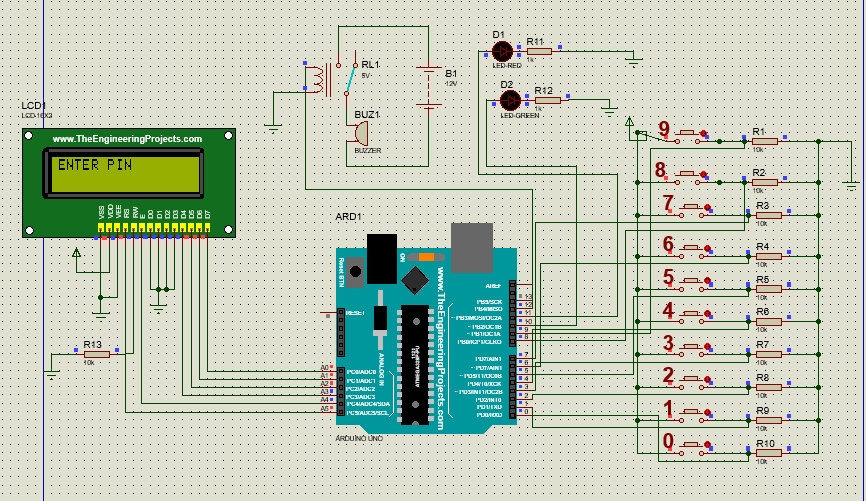
\includegraphics[scale=0.7]{schematic1.png}
\caption{\textbf{Schematic}}
\label{schematic_diagram1}
\end{figure}
 
\pagebreak

\begin{center}
\section*{PROJECT - 2}
\section*{\textbf{Calculator Using Arduino UNO}}
 \addcontentsline{toc}{section}{2. Calculator Using Arduino UNO}
\end{center}

\subsection*{\textbf{Description :}}
 \addcontentsline{toc}{subsection}{Description}
 
 This Project is to design Calculator using Arduino UNO board, 4x4 Keypad and a LCD display. This calculator do basic mathematical operations like Addition (+), Subtraction (-), Multiplication (x), and Division (/). When the user enters the operands in the LCD and based on the operator the operation need to be performed (i.e. when user enters operator “+” in the keypad then addition operation need to be performed and follows…). The calculator will take only two operands and single operator at a time. The calculator takes recent two operators and recent operand only.

 
 \subsection*{\textbf{Block Diagram :}}
 \addcontentsline{toc}{subsection}{Block Diagram}
 
 \begin{figure}[h]
\centering
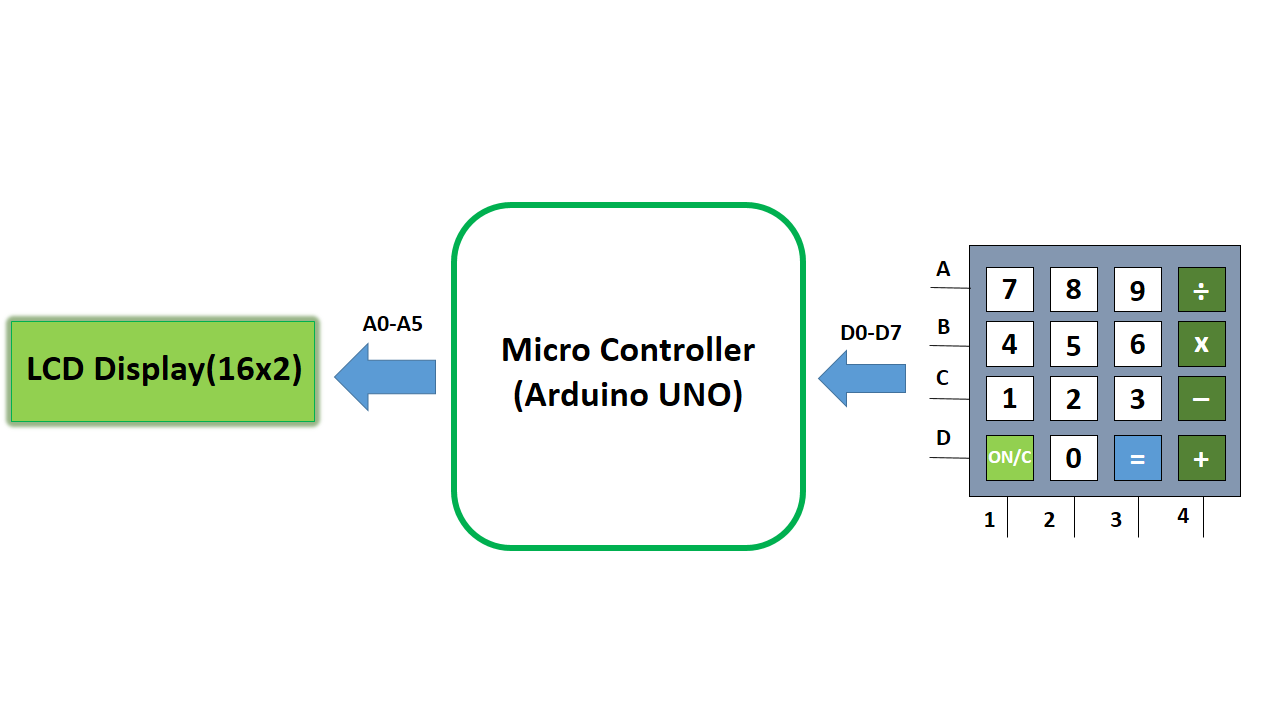
\includegraphics[scale=0.5]{block2.png}
\caption{\textbf{Block Diagram}}
\label{block_diagram1}
\end{figure} 
 
 \subsection*{\textbf{Input and Output :}}
 \addcontentsline{toc}{subsection}{Input and Output}
 
  \begin{tabular}{|c|c|c|c|c|c|c|}
  \hline
 \textbf{S.No }& \textbf{Description} & \textbf{Name}&\textbf{Type }& \textbf{Data Direction}  &\textbf{ Spec}& \textbf{Remarks} \\
  \hline
  1 & KeyPad Row1 Pin & A & INP  & DI  &5VDC&Active High \\
  \hline
  2 & KeyPad Row2 Pin  &B&INP  & DI  &5VDC&Active High \\
  \hline
  3 &  KeyPad Row3 Pin  & C &INP &DI &5VDC&Active High \\
  \hline
  4 & KeyPad Row4 Pin  & D &INP & DI  & 5VDC&Active High \\
  \hline
  5&KeyPad Column 1 Pin & 1 &INP &DI &5VDC&Active High\\
 \hline
  6 & KeyPad Column 2 Pin& 2 &INP &DI &5VDC&Active High \\
  \hline
  7 &  KeyPad Column 3 Pin & 3 &INP & DI  &5VDC&Active High\\
  \hline
   8 &KeyPad Column 4 Pin& 4 &INP  & DI &5VDC&Active High \\
  \hline
  9 &LCD Reset Pin & RS &OUT &DO&5VDC&Active High \\
  \hline
  10 &LCD Enable Pin & E &OUT &DO &5VDC&Active High \\
  \hline
  11 &LCD Data Pin 1 & D4 &OUT &DO &5VDC&Active High \\
  \hline
  12 & LCD Data Pin 2& D5 &OUT & DO &5VDC&Active High \\
 \hline
  13 & LCD Data Pin 3 & D6 &OUT & DO &5VDC&Active High \\
  \hline
  14 &LCD Data Pin 4 & D7 &OUT& DO &5VDC&Active High \\
  \hline
\end{tabular}
 
 \subsection*{\textbf{Source Code :}}
 \addcontentsline{toc}{subsection}{Source Code}
  \begin{lstlisting}[language=C] 
  
 #include <LiquidCrystal.h>
 #include <Keypad.h>
   
const byte ROWS = 4;
const byte COLS = 4;
//char Operator[15]; 

char keys[ROWS][COLS] = {

                          {'7','8','9','D'},

                          {'4','5','6','C'},

                          {'1','2','3','B'},

                          {'*','0','#','A'}

                        };

byte rowPins[ROWS] = {A0, A1, A2, A3}; 
byte colPins[COLS] = {1, 2, 3, 4};

Keypad kpd = Keypad( makeKeymap(keys), rowPins, colPins, ROWS, COLS );

LiquidCrystal lcd(13, 12, 11, 10, 9, 8);
long operand1,operand2,final_Result;
int operand;
char key,Operator;
bool operater_Notpressed,result,key_Operator;
void key_Pressed();
void operand_Calculation();
void result_Calculation();

void setup() 
{
  operand1=0;
  operand2=0;
  operand=0;
  final_Result=0;
  operater_Notpressed = true;
  result = false;
  lcd.begin(16,2);
  lcd.print("Calculator");
  lcd.setCursor(0,1);
  lcd.print("By Sai Krishna");
  delay(2000);
  lcd.clear();
}

void loop()
{
  key = kpd.getKey();
  if(key!=NO_KEY)
  {
    key_Pressed();
    operand_Calculation();
  }
  if(result==true)
  {
    result_Calculation();
  }
}

void key_Pressed()
{
  if(key=='0'||key=='1'||key=='2'||key=='3'
  ||key=='4'||key=='5'||key=='6'||key=='7'||
  key=='8'||key=='9')
  { 
    key_Operator=false;  
    if(key=='1')
    {
      operand = 1;
    }
    if(key=='2')
    {
      operand = 2;
    }
    if(key=='3')
    {
      operand = 3;
    }
    if(key=='4')
    {
      operand = 4;
    }
    if(key=='5')
    {
      operand = 5;
    } 
    if(key=='6')
    {
      operand = 6;
    }
    if(key=='7')
    {
      operand = 7;
    } 
    if(key=='8')
    {
      operand = 8;
    }
    if(key=='9')
    {
      operand = 9;
    }
    if(key=='0')
    {
      operand = 0;
    }
    lcd.print(operand);
  }
  
  else if(key=='A'||key=='B'||key=='C'||key=='D')
  {
    operater_Notpressed = false;
    key_Operator=true;    
    if(key=='A')
    {
      Operator='+';
    }
    if(key=='B')
    {
      Operator='-';
    }
    if(key=='C')
    {
      Operator='x';
    }
    if(key=='D')
    {
      Operator='/';
    }
    lcd.print(Operator);   
  }
  
  else if(key=='#')
  { 
    key_Operator=false;   
    result = true;
    lcd.print('=');
  }
  else
  {    
    reset(); //Clear all the numbers
    lcd.clear();
  }    
}

void operand_Calculation()
{
  if(operater_Notpressed == true)
  {
    operand1=(operand1*10)+operand;
  }
  else
  {
    if(result!=true && key_Operator!=true)
    {
      operand2=(operand2*10)+operand;
    }
  }

}
void result_Calculation()
{
    if(Operator=='+')
    {
      final_Result = operand1 + operand2;
    }
    if(Operator=='-')
    {
      final_Result = operand1 - operand2;
    }
    if(Operator=='x')
    {
      final_Result = operand1 * operand2;
    }
    if(Operator=='/')
    {
      final_Result = operand1 / operand2;
    }
    lcd.setCursor(0,1);
    lcd.print(final_Result); 
}
void reset()
{
  operand1=0;
  operand2=0;
  operand=0;
  final_Result=0;
  operater_Notpressed = true;
  key_Operator=false;
  result = false;
}
 \end{lstlisting}
 
  \subsection*{\textbf{Circuit or Schematic :}}
 \addcontentsline{toc}{subsection}{Circuit or Schematic}
 
   \begin{figure}[h]
\centering
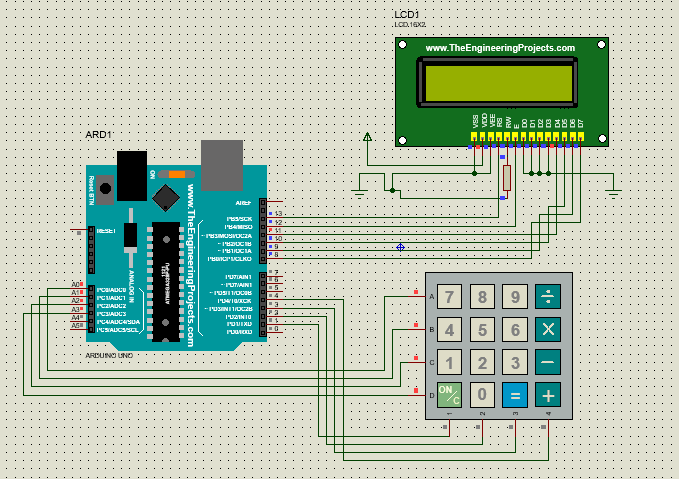
\includegraphics[scale=0.7]{schematic2.png}
\caption{\textbf{Schematic}}
\label{schematic_diagram1}
\end{figure}
 
\pagebreak

\begin{center}
\section*{PROJECT - 3}
\section*{\textbf{Display Date And Time Using RTC module}}
 \addcontentsline{toc}{section}{3. Display Date And Time Using RTC module}
\end{center}

\subsection*{\textbf{Description :}}
 \addcontentsline{toc}{subsection}{Description}
 This Project is to display Date and Time using Real Time Clock (RTC) on a LCD (16x2) display. The RTC module is used to keep track of the time even when the Arduino board is powered off. The time data from the RTC module is then displayed on the LCD display using I2C communication. A library is used to simplify the code and make it easier to work with the RTC and LCD components. The date and time in the code can be adjusted before uploading it to the board to ensure that the correct time is displayed.
 
 \subsection*{\textbf{Block Diagram :}}
 \addcontentsline{toc}{subsection}{Block Diagram}
 
  \begin{figure}[h]
\centering
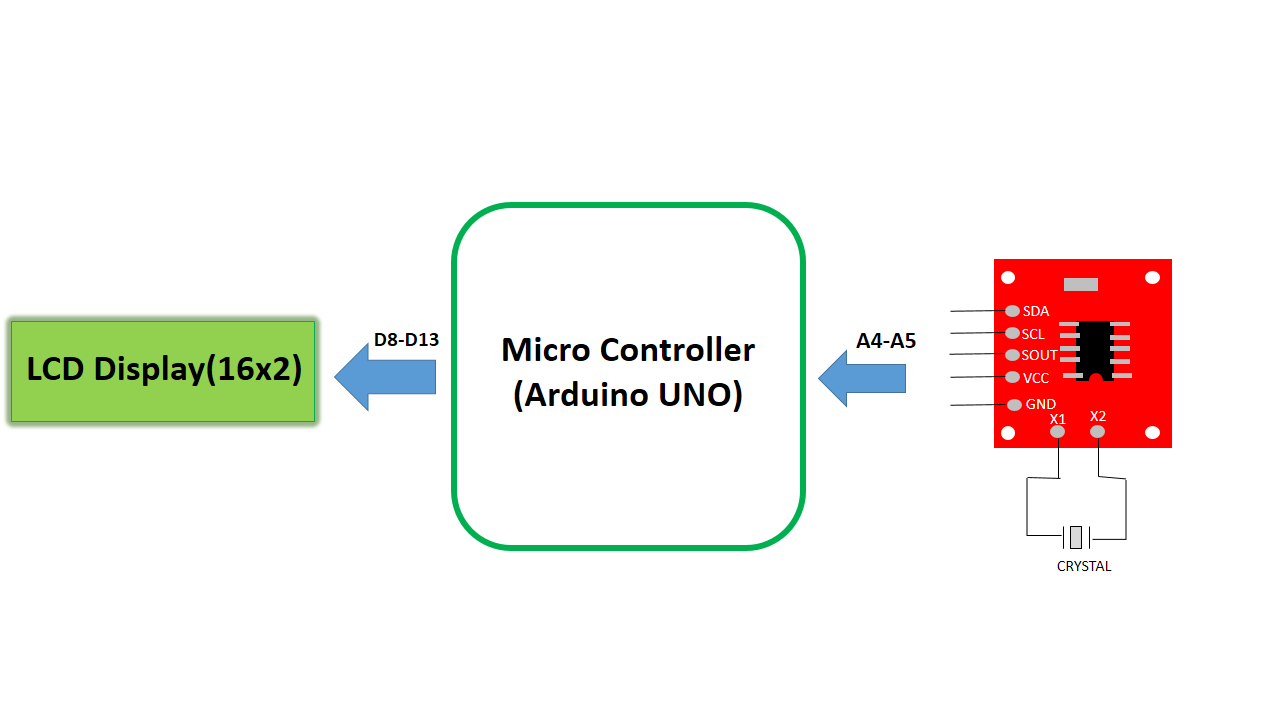
\includegraphics[scale=0.5]{block3.png}
\caption{\textbf{Block Diagram}}
\label{block_diagram1}
\end{figure} 
 
 \subsection*{\textbf{Input and Output :}}
 \addcontentsline{toc}{subsection}{Input and Output}
 
   \begin{tabular}{|c|c|c|c|c|c|c|}
  \hline
 \textbf{S.No }& \textbf{Description} & \textbf{Name}&\textbf{Type }& \textbf{Data Direction}  &\textbf{ Spec}& \textbf{Remarks} \\
  \hline
  1 &Serial Data &SDA & INP  & DI  &5VDC&Active High \\
  \hline
  2 &Serial Clock &SCL&INP  & DI  &5VDC&Active High \\
  \hline
  3 &LCD Reset Pin & RS &OUT &DO&5VDC&Active High \\
  \hline
  4 &LCD Enable Pin & E &OUT &DO &5VDC&Active High \\
  \hline
  5&LCD Data Pin 1 & D4 &OUT &DO &5VDC&Active High \\
  \hline
  6 & LCD Data Pin 2& D5 &OUT & DO &5VDC&Active High \\
 \hline
  7 & LCD Data Pin 3 & D6 &OUT & DO &5VDC&Active High \\
  \hline
  8 &LCD Data Pin 4 & D7 &OUT& DO &5VDC&Active High \\
  \hline
\end{tabular}
 
 \subsection*{\textbf{Source Code :}}
 \addcontentsline{toc}{subsection}{Source Code}
  \begin{lstlisting}[language=C] 
 #include <LiquidCrystal.h>
 #include <Wire.h>
 #include "RTClib.h"

 RTC_DS1307 rtc;
 LiquidCrystal lcd(13, 12, 11, 10, 9, 8);

 void setup()
  {
  lcd.begin(16, 2);
  lcd.print("Initializing RTC...");
  if (! rtc.begin()) {
    lcd.setCursor(0, 1);
    lcd.print("RTC failed");
    while (1);
  }
  if (! rtc.isrunning())
   {
    lcd.setCursor(0, 1);
    lcd.print("RTC is NOT running");
    while (1);
  }
  lcd.clear();
}

void loop()
 {
  DateTime now = rtc.now();
  lcd.setCursor(0, 0);
  lcd.print(now.day(), DEC);  
  lcd.print('/');
  lcd.print(now.month(), DEC);
  lcd.print('/');
  lcd.print(now.year(), DEC);
  lcd.setCursor(0, 1);
  lcd.print(now.hour(), DEC);
  lcd.print(':');
  lcd.print(now.minute(), DEC);
  lcd.print(':');
  lcd.print(now.second(), DEC);
  delay(1000);
}
 \end{lstlisting}
 
  \subsection*{\textbf{Circuit or Schematic :}}
 \addcontentsline{toc}{subsection}{Circuit or Schematic} 
 
    \begin{figure}[h]
\centering
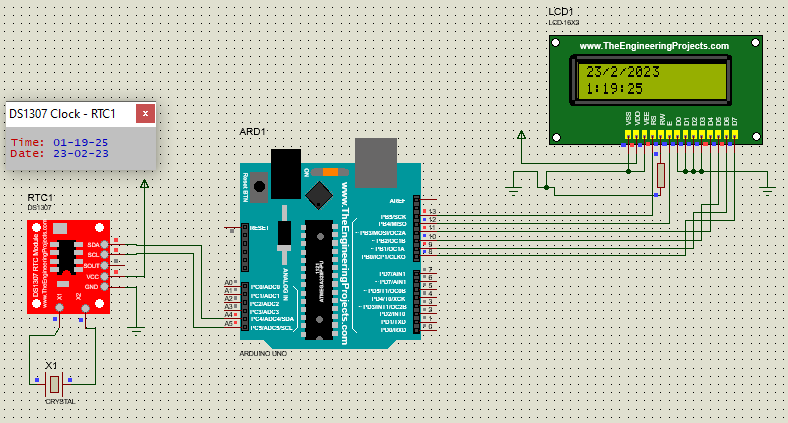
\includegraphics[scale=0.7]{schematic3.png}
\caption{\textbf{Schematic}}
\label{schematic_diagram3}
\end{figure}
 
\pagebreak

\begin{center}
\section*{PROJECT - 4}
\section*{\textbf{Designing EEPROM based Counting Industry  product}}
 \addcontentsline{toc}{section}{4. Designing EEPROM based Counting Industry  product}
\end{center}

\subsection*{\textbf{Description :}}
 \addcontentsline{toc}{subsection}{Description}
 This Project is to store count of Good products and Bad Products which are passing on a convener belt in an Industry in EEPROM and display the stored data on a LCD (20x4) display. EEPROM stands for Electrically Erasable Programmable Read-Only Memory. It is a type of non-volatile memory that can be programmed and erased electronically. EEPROMs are used to store small amounts of data that must be retained even when the power is turned off.The Arduino takes inputs from the good and bad product detection sensors and write the data in EEPROM, the written data is visible and monitored using serial monitor. The count is displayed in 20x4 LCD.
 \subsection*{\textbf{Block Diagram :}}
 \addcontentsline{toc}{subsection}{Block Diagram}
 
  \begin{figure}[h]
\centering
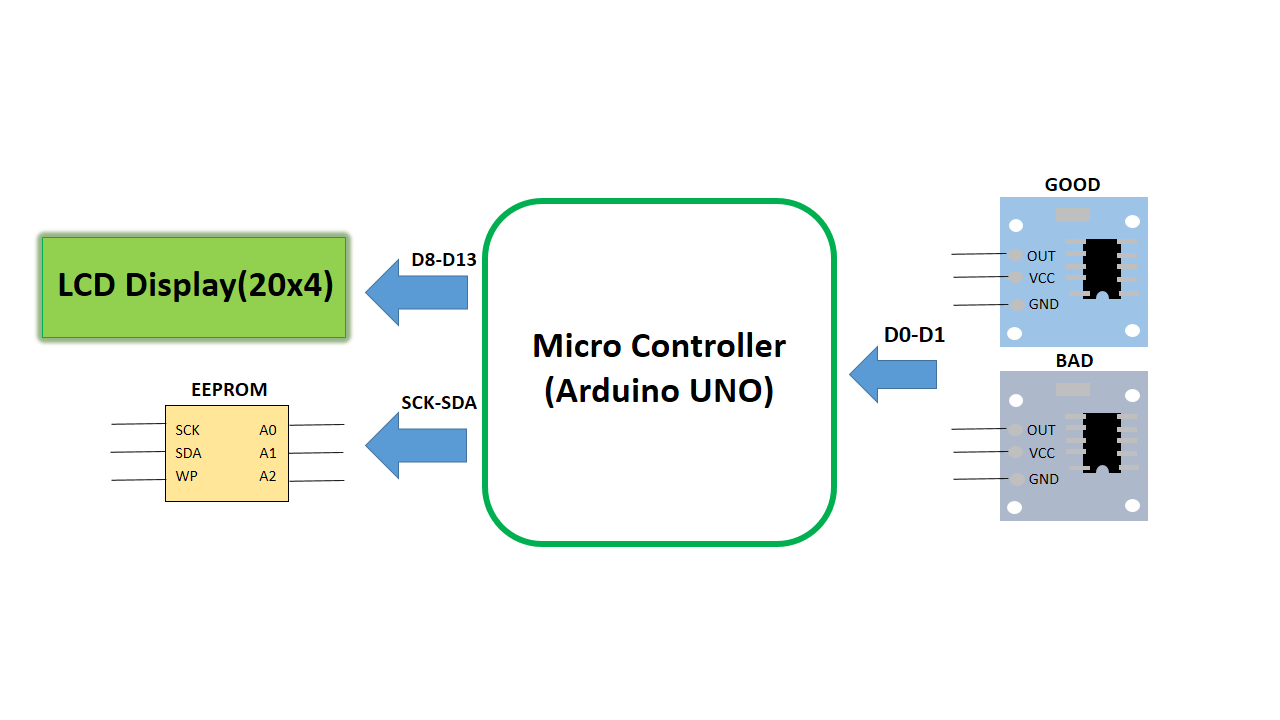
\includegraphics[scale=0.5]{block4.png}
\caption{\textbf{Block Diagram}}
\label{block_diagram4}
\end{figure} 
 
 \subsection*{\textbf{Input and Output :}}
 \addcontentsline{toc}{subsection}{Input and Output}
 
   \begin{tabular}{|c|c|c|c|c|c|c|}
  \hline
 \textbf{S.No }& \textbf{Description} & \textbf{Name}&\textbf{Type }& \textbf{Data Direction}  &\textbf{ Spec}& \textbf{Remarks} \\
  \hline
  1 & GOOD Product Pin & D0 & INP  & DI  &5VDC&Active High \\
  \hline
  2 & BAD Product Pin  &D1&INP  & DI  &5VDC&Active High \\
  \hline
  3 & EEPROM SCK Pin  & SCK &OUT &DO &5VDC&Active High \\
  \hline
  4 & EEPROM SDA Pin  & SDA &OUT & DO  & 5VDC&Active High \\
  \hline
  5 &LCD Reset Pin & RS &OUT &DO&5VDC&Active High \\
  \hline
  6 &LCD Enable Pin & E &OUT &DO &5VDC&Active High \\
  \hline
  7 &LCD Data Pin 1 & D4 &OUT &DO &5VDC&Active High \\
  \hline
  8 & LCD Data Pin 2& D5 &OUT & DO &5VDC&Active High \\
 \hline
  9 & LCD Data Pin 3 & D6 &OUT & DO &5VDC&Active High \\
  \hline
  10 &LCD Data Pin 4 & D7 &OUT& DO &5VDC&Active High \\
  \hline
\end{tabular}
 
 \subsection*{\textbf{Source Code :}}
 \addcontentsline{toc}{subsection}{Source Code}
  \begin{lstlisting}[language=C] 
#include <Wire.h>
#include <LiquidCrystal.h>

#define TotalAddress 0x00
#define GoodAddress 0x0C
#define BadAddress 0x18 

int bad = 0;
int good = 0;
int total = 0;
const int eeprom_address = 0x50;  
void LCD_print();
void Clear_EEPROM();

LiquidCrystal lcd(4, 5, 6, 7, 8, 9);

void setup() 
{
  Wire.begin();
  Serial.begin(9600);
  for(int i=2 ; i<4 ; i++)
  {
    pinMode(i , INPUT);
  }

  pinMode(10 , INPUT);
  
  lcd.begin(20, 4);
  lcd.print("--Working of EEPROM--");
  lcd.setCursor(0, 1);
  lcd.print("        By         ");
  lcd.setCursor(0, 2);
  lcd.print(" SAI KRISHNA DASARI ");  
  delay(2000);
  lcd.clear();

  for (int address = 0; address < 36; address++)
  {
    writeEEPROM(TotalAddress+address, 0xFF);
  }
  
}

void loop() 
{

  int clearROM = digitalRead(10);
  
  if(!clearROM) //clears EEPROM when it returns 0
  {
    Clear_EEPROM(); //clear the EEPROM
  }
  
  else
  {
    if(digitalRead(2))
    {
      good++;
    }
    if(digitalRead(3))
    {
      bad++;
    }
    total = good + bad ;
    LCD_print();
    
    byte i = 0x00 ;
    for(int num = total ; num > 0 ; num = num/10)
    {
      int rem = num % 10 ;
      writeEEPROM(TotalAddress+i, rem); 
      
      Serial.print(" Written Total Products at: ");
      Serial.print(TotalAddress+i);
      Serial.print(" is ");
      Serial.println(rem);

      
      i++;
    }

    byte j = 0x00 ;
    for(int num = good ; num > 0 ; num = num/10)
    {
      int rem = num % 10 ;
      writeEEPROM(GoodAddress+j, rem);
      
      Serial.print(" Written Good Products at:");
      Serial.print(GoodAddress+j);
      Serial.print(" is ");
      Serial.println(rem);
      
      j++;
    }
    
    byte k = 0x00 ;
    for(int num = bad ; num > 0 ; num = num/10)
    {
      int rem = num % 10 ;
      writeEEPROM(BadAddress+k, rem);
      
      Serial.print(" Written Bad Products at: ");
      Serial.print(BadAddress+k);
      Serial.print(" is ");
      Serial.println(rem);
      
      k++;
    }                 
  }  
    
  delay(500);

}

byte readEEPROM(int address) 
{
  byte data;
  Wire.beginTransmission(eeprom_address);
  Wire.write((int)(address >> 8)); 
  Wire.write((int)(address & 0xFF));
  Wire.endTransmission();
  Wire.requestFrom(eeprom_address, 1);
  if (Wire.available()) 
  {
    data = Wire.read();
  }
  return data;
}

void writeEEPROM(int address, byte data) {
  Wire.beginTransmission(eeprom_address);
  Wire.write((int)(address >> 8)); 
  Wire.write((int)(address & 0xFF)); 
  Wire.write(data);
  Wire.endTransmission();
  delay(5);  
}

void LCD_print()
{
  lcd.clear();
  
  lcd.setCursor(0, 2);
  lcd.print("BAD Products : ");
  lcd.print(bad);

  lcd.setCursor(0, 3);
  lcd.print("GOOD Products : ");
  lcd.print(good);
  
  lcd.setCursor(0, 0);
  lcd.print("TOTAL PRODUCTS : ");
  lcd.print(total);
  lcd.setCursor(0, 1);
  lcd.print(total);

}
void Clear_EEPROM()
{
   for (int address = 0; address < 32768; address++) 
   {
    Wire.beginTransmission(eeprom_address);
    Wire.write((int)(address >> 8));
    Wire.write((int)(address & 0xFF));
    Wire.write(0xFF);
    Wire.endTransmission();
  }

    Serial.println("EEPROM data cleared!");  
}


 \end{lstlisting}
 
  \subsection*{\textbf{Circuit or Schematic :}}
 \addcontentsline{toc}{subsection}{Circuit or Schematic}  
 
    \begin{figure}[h]
\centering
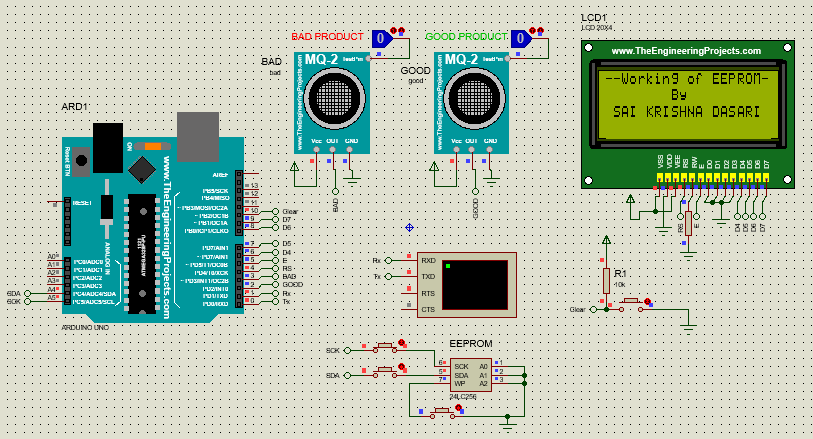
\includegraphics[scale=0.7]{schematic4.png}
\caption{\textbf{Schematic}}
\label{schematic_diagram4}
\end{figure}
 
 \pagebreak

\begin{center}
\section*{PROJECT - 5}
\section*{\textbf{Automatic Washing Machine using Arduino UNO}}
 \addcontentsline{toc}{section}{5. Automatic Washing Machine using Arduino UNO}
\end{center}

\subsection*{\textbf{Description :}}
 \addcontentsline{toc}{subsection}{Description}
  This Project is create fully automatic Washing Machine using Arduino UNO and display the functioning on a LCD (20x4) display. The washing machine consist of Drain switch ,User Timer Module, Realy, Motor, Buzzer, LCD Display.The User Timer Module is used to provide the user interface.The drain switch is used to detect the water level.Relay will automatically close the drain switch when the all water is drained. Motor Rotation indicates the washing of the clothes. Buzzer will blow when the washing is completed. 
 \subsection*{\textbf{Block Diagram :}}
 \addcontentsline{toc}{subsection}{Block Diagram}
 
  \begin{figure}[h]
\centering
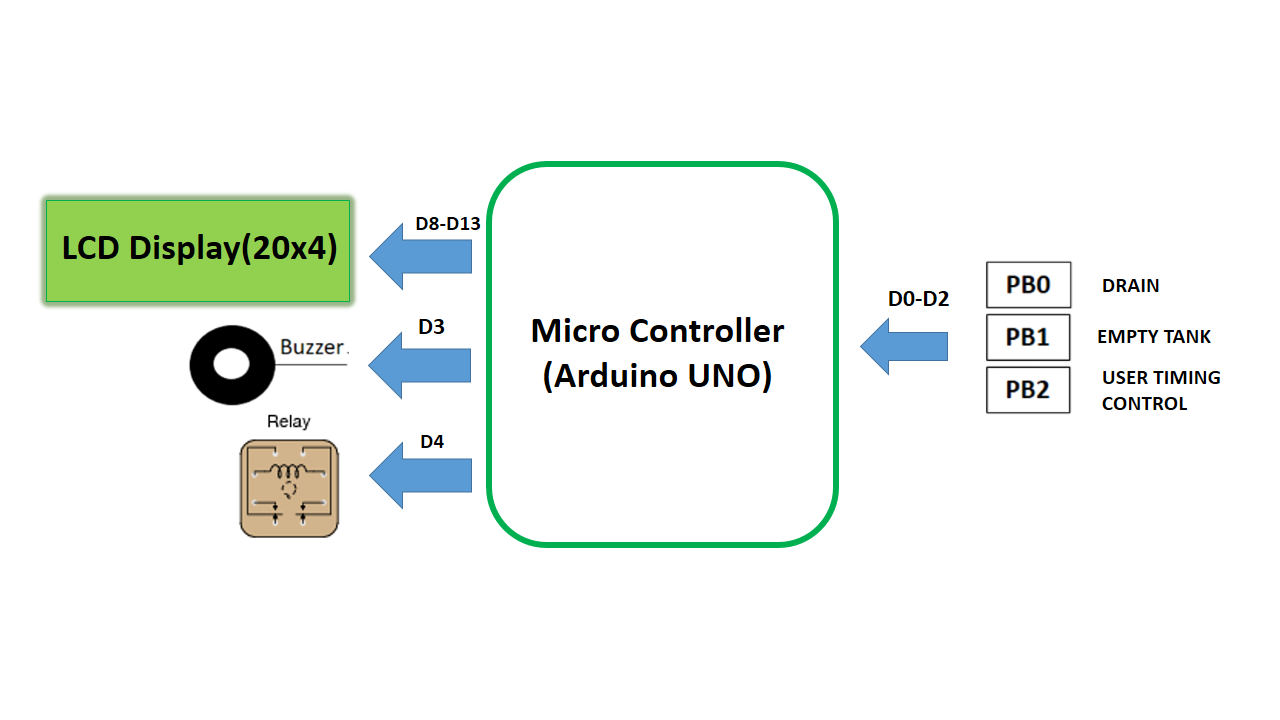
\includegraphics[scale=0.4]{block5.png}
\caption{\textbf{Block Diagram}}
\label{block_diagram5}
\end{figure} 
 
 \subsection*{\textbf{Input and Output :}}
 \addcontentsline{toc}{subsection}{Input and Output}
 
   \begin{tabular}{|c|c|c|c|c|c|c|}
  \hline
 \textbf{S.No }& \textbf{Description} & \textbf{Name}&\textbf{Type }& \textbf{Data Direction}  &\textbf{ Spec}& \textbf{Remarks} \\
  \hline
  1 & Drain Pin & PB0 & INP  & DI  &5VDC&Active High \\
  \hline
  2 & Empty Tank Pin  &PB1&INP  & DI  &5VDC&Active High \\
  \hline
  3 &  User Timing Control  & PB2 &INP &DI &5VDC&Active High \\
  \hline
  4 & Relay  Pin  & D4  &OUT & DO  & 5VDC&Active High \\
  \hline
  5&Buzzer Pin & D3 &OUT & DO  &5VDC&Active High\\
 \hline
  6 &LCD Reset Pin & RS &OUT &DO&5VDC&Active High \\
  \hline
  7 &LCD Enable Pin & E &OUT &DO &5VDC&Active High \\
  \hline
  8 &LCD Data Pin 1 & D4 &OUT &DO &5VDC&Active High \\
  \hline
  9 & LCD Data Pin 2& D5 &OUT & DO &5VDC&Active High \\
 \hline
  10 & LCD Data Pin 3 & D6 &OUT & DO &5VDC&Active High \\
  \hline
  11 &LCD Data Pin 4 & D7 &OUT& DO &5VDC&Active High \\
  \hline
\end{tabular}
 
 \subsection*{\textbf{Source Code :}}
 \addcontentsline{toc}{subsection}{Source Code}
  \begin{lstlisting}[language=C] 
#include <LiquidCrystal.h>

const int next = A1;
const int motorPin = 13;
const int select = A0;
const int drainPin = 2;
const int emptyWaterSwitch = 3;
const int relayPin = 7; // output pin for relay
const int buzzerPin = 8; // output pin for buzzer
const int lcdRsPin = 12; // LCD RS pin
const int lcdEnPin = 11; // LCD EN pin
const int lcdD4Pin = 5; // LCD D4 pin
const int lcdD5Pin = 4; // LCD D5 pin
const int lcdD6Pin = 9; // LCD D6 pin
const int lcdD7Pin = 10; // LCD D7 pin
LiquidCrystal lcd(lcdRsPin, lcdEnPin,
 lcdD4Pin, lcdD5Pin, lcdD6Pin, lcdD7Pin);

void setup()
 {
  pinMode(drainPin, INPUT);
  pinMode(emptyWaterSwitch, INPUT);
  pinMode(relayPin, OUTPUT);
  pinMode(motorPin, OUTPUT);
  pinMode(buzzerPin, OUTPUT);
  pinMode(A0, INPUT);
  pinMode(A1, INPUT);

  lcd.begin(20, 4); // Initialize 20x4 LCD
  lcd.clear(); // Clear the LCD display
  lcd.print("Washing Machine"); 
  delay(2000);
}

void loop() {
  // Check if drain switch is closed
  while (digitalRead(drainPin) == LOW) 
  {
    // Wait for water to drain out
    lcd.clear();
    lcd.print("Waiting to Drain...");
    delay(500);
  }
  digitalWrite(relayPin, HIGH);

  // Check empty water tank switch
  if (digitalRead(emptyWaterSwitch) == HIGH) 
  {
    // Turn on relay to close drain valve
    lcd.setCursor(0, 1);
    lcd.print("Empty switch is Pressed");   
    digitalWrite(relayPin, HIGH);
    lcd.setCursor(0, 2);
    lcd.print("Relay Turned ON...");
    lcd.setCursor(0, 3);
    lcd.print("Drain Closed...");
  

  // Ask user to set washing timer value
  lcd.clear();
  lcd.print("Set washing time:");
  lcd.setCursor(3,1);
  lcd.print("30 Min");
  lcd.setCursor(3,2);
  lcd.print("45 Min");
  lcd.setCursor(3,3);
  lcd.print("60 Min");
  int washingTime = 0;
  int count = 0;

  while(!digitalRead(select))
  {
    if(digitalRead(next))
    {
      count = count + 1;
      delay(500);
    }
    else
    {
      if(count==1)
      {
        lcd.clear();
        lcd.setCursor(0,1);
        lcd.print("-->");
        lcd.setCursor(3,1);
        lcd.print("30 Min");
        lcd.setCursor(3,2);
        lcd.print("45 Min");
        lcd.setCursor(3,3);
        lcd.print("60 Min");
        washingTime = 2000;        
      }
      else if(count==2)
      {
        lcd.clear();
        lcd.setCursor(0,2);
        lcd.print("-->");
        lcd.setCursor(3,1);
        lcd.print("30 Min");
        lcd.setCursor(3,2);
        lcd.print("45 Min");
        lcd.setCursor(3,3);
        lcd.print("60 Min");
        washingTime = 4000; 
      }
      else if(count==3)
      {
        lcd.clear();
        lcd.setCursor(0,3);
        lcd.print("-->") ;
        lcd.setCursor(3,1);
        lcd.print("30 Min");
        lcd.setCursor(3,2);
        lcd.print("45 Min");
        lcd.setCursor(3,3);
        lcd.print("60 Min");
        washingTime = 6000;
      }    
      
      else if(count>=4)
      {
        count = 1;
      }
      else
      {
        count = 0;
      }  
    }
    delay(500);
  } 
   

  // Run washing motor till timer time elapses
  lcd.clear();
  lcd.print("Washing.....");
  
  int elapsed = 0;
  digitalWrite(motorPin, HIGH);
      
  while (elapsed < washingTime)
   {
    delay(1000); // Delay 1 second
    elapsed += 1000;
  }
  digitalWrite(motorPin, LOW);

  // Open drain valve to drain water
  lcd.clear();
  lcd.print("Draining water");
  digitalWrite(relayPin, LOW);
  
  while (!digitalRead(drainPin))
   {
    digitalWrite(buzzerPin, HIGH);
    delay(500);
    digitalWrite(buzzerPin, LOW);
    delay(500);
  }

  // Close drain valve
  lcd.clear();
  lcd.setCursor(3,2);
  lcd.print("Washing COMPLETED");
  digitalWrite(relayPin, HIGH);
  delay(3000); // Delay 5 minutes

  digitalWrite(buzzerPin, HIGH);
  delay(2000);
  digitalWrite(buzzerPin, LOW);
  digitalWrite(relayPin, LOW);  
}

else
{
   lcd.clear();
  lcd.print("Waiting for Tank to Empty"); 
  delay(200)  ;
}
}

 
 \end{lstlisting}
 \pagebreak
  \subsection*{\textbf{Circuit or Schematic :}}
 \addcontentsline{toc}{subsection}{Circuit or Schematic}
 
    \begin{figure}[h]
\centering
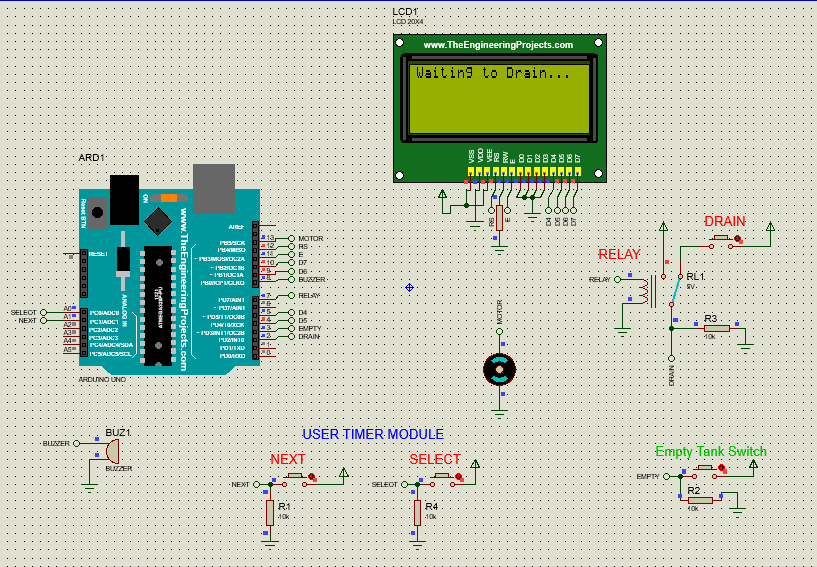
\includegraphics[scale=0.7]{schematic5.png}
\caption{\textbf{Schematic}}
\label{schematic_diagram5}
\end{figure}
 
\pagebreak
\begin{center}
\section*{How to Showcase on GitHub?}
\addcontentsline{toc}{section}{How to Showcase on GitHub?}
\end{center}
When creating and uploading your projects to GitHub, it's important to follow some best practices to ensure that your work is easy to understand and use for others. Here are some key patterns you should follow:\\

\textbf{Organize your code:} Use clear and concise names for your files and directories, and create a logical directory structure to make it easy for others to navigate your code. Use comments to explain what your code does and how it works.\\

\textbf{Use a consistent style:} Follow a consistent coding style throughout your project, including indentation, spacing, and naming conventions. This makes your code more readable and easier to understand.\\

\textbf{Use version control:} Use Git to manage changes to your code over time, and make frequent commits to keep a detailed history of your work.\\

\textbf{Include a README:} Write a clear and concise README file that explains what your project does, how to install and use it, and any other relevant information that others might need to know.\\

\textbf{Use descriptive commit messages:} Write clear and descriptive commit messages that explain the changes you made and why you made them.\\

By following these patterns, you can create high-quality projects on GitHub that are easy to understand and use for others. This can help you gain recognition from others in your field, and can demonstrate your technical skills to potential employers.
\\
\subsection*{Key Components for Strong Technical Portfolios}
 \addcontentsline{toc}{subsection}{Key Components for Strong Technical Portfolios}
including documentation, firmware, and hardware folders in your GitHub repository can be a good way to make it easy for interviewers to review your technical projects.
\pagebreak
\subsubsection*{Documentation:} 
 \addcontentsline{toc}{subsubsection}{Documentation:}
Include a folder for documentation that describes what your project does, how it works, and any instructions on how to use it. This can be in the form of a README file or additional documentation files in a separate folder. Make sure that your documentation is clear and well-organized, so that anyone reviewing your project can easily understand what you've built.

\subsubsection*{Firmware:}
 \addcontentsline{toc}{subsubsection}{Firmware:}
 If your project involves firmware (e.g. for an embedded system), include a folder that contains the source code for your firmware. Make sure that your code is well-organized and includes comments to explain what each part of the code does.

\subsubsection*{Hardware:}
 \addcontentsline{toc}{subsubsection}{Hardware:}
 If your project involves any hardware components, include a folder that contains any schematics, diagrams, or other files related to the hardware. This can help reviewers understand how the hardware components fit together and how they interact with the firmware.\\

By including these components in your GitHub repository, you can make it easy for interviewers to review your project and gain a better understanding of your technical skills. It also demonstrates your attention to detail and commitment to creating high-quality projects.
\pagebreak
\section*{Student Feedback}
\addcontentsline{toc}{section}{Student Feedback}
Learning is the process of life and being student of this trust is so special part of my life.Thanks to all teachers who guided me in this course and in extra curricular activities. Special thanks to my trainer who taught this topic so easily. This experience will help me grow my future in every direction and serve the needs of society as best as possible.
\section*{Uniqueness of the Course}
\addcontentsline{toc}{section}{Uniqueness of the Course}
This course teaches in depth of Embedded Systems and Arduino where institutions fail to teach. I have gained so much confidence while asking doubts to know answers in depth because the trainer is friendly and supportive.

\section*{Concluding Remarks}
\addcontentsline{toc}{section}{Concluding Remarks}
Sure trust is not just a trust but it’s a family where each and every student is getting help in every manner. Being member of this trust i have tried to contribute in every manner. Students from different places meet here and help each other. In future i will do my level best in growing this trust.
\\
\vspace{1.4in}
\begin{center}
\line(1,0){60}
{\Large \textbf{THE END}}
\line(1,0){60}
\end{center}
\end{document}
